\documentclass[conference]{IEEEtran}
\usepackage{amsmath,amssymb,graphicx,booktabs,array,url,xcolor}
\usepackage[hidelinks]{hyperref}
\newcommand{\ind}{\mathbf{1}}
\newcommand{\Count}{\operatorname{COUNT}}
\hyphenation{joint NousDB near context claim singleton strict}
\newcolumntype{P}[1]{>{\raggedright\arraybackslash}p{#1}}
\graphicspath{{../figures/}}
\hypersetup{
pdftitle={[Experiment, Analysis, and Benchmark] Auditing Batched Semantic COUNT: Fidelity Checks and Full Policy Cost},
pdfauthor={Zida Yang; Kangzheng Peng; Guquan You; Yongjun Dai; Chenhang He; Zijian Wang; Jiexin Zheng; Cong Wang; Xiaolong Shi},
pdfsubject={Experiment, Analysis, and Benchmark},
pdfkeywords={semantic query processing; large language models; COUNT; fidelity certification; prefix caching; query optimization}
}
\begin{document}
\title{[Experiment, Analysis, and Benchmark]\\Auditing Batched Semantic COUNT:\\Fidelity Checks and Full Policy Cost}
\author{
\IEEEauthorblockN{\href{https://orcid.org/0009-0000-2386-2533}{Zida Yang}\textsuperscript{1,*}, \href{https://orcid.org/0009-0005-1960-6488}{Kangzheng Peng}\textsuperscript{2,*},
\href{https://orcid.org/0009-0005-5915-7058}{Guquan You}\textsuperscript{3,*}, \href{https://orcid.org/0009-0005-7049-2607}{Yongjun Dai}\textsuperscript{4,*}, \href{https://orcid.org/0009-0001-9002-0974}{Chenhang He}\textsuperscript{2},\\
 \href{https://orcid.org/0009-0001-8267-7247}{Zijian Wang}\textsuperscript{2}, \href{https://orcid.org/0009-0005-5838-0135}{Jiexin Zheng}\textsuperscript{1,\textdagger}, \href{https://orcid.org/0000-0002-5300-0122}{Cong Wang}\textsuperscript{1,\textdagger}}
\IEEEauthorblockA{
\textsuperscript{1}Guanghua School of Management, Peking University, Beijing, China\\
\textsuperscript{2}School of Artificial Intelligence, Guangzhou University, Guangzhou, China\\
\textsuperscript{3}Institute of Emergency Safety Innovations, Guangzhou University, Guangzhou, China\\
\textsuperscript{4}Institute of Computing Science and Technology, Guangzhou University, Guangzhou, China\\
\texttt{2401111090@stu.pku.edu.cn, pkz6@qq.com, youguquan@gzhu.edu.cn}\\
\texttt{1112433026@e.gzhu.edu.cn, 18221681139@139.com, 2209744955@qq.com}\\
\texttt{jiexinzheng@gsm.pku.edu.cn, wangcong@gsm.pku.edu.cn}\\
\textsuperscript{*}The first four authors contributed equally and share first authorship.\\
\textsuperscript{\textdagger}Corresponding authors: Cong Wang and Jiexin Zheng.
}}

\maketitle
\begin{abstract}
Semantic COUNT applies a language-model filter to rows and counts the positive labels. Batching several rows in one request can save calls, but an optimizer may first pay to check whether their labels change. We audit that complete decision by following an existing fidelity check through size selection, full execution and fallback, and measuring the returned result and the cost of every stage. Native LOTUS and a declared custom batch operator are evaluated in 36 configurations over six workloads, two domains and two models, with 16 further policies comparing probe budgets. In the sole accepted batch deployment, all 80 check comparisons agree and full-result disagreement remains below 5\%; nevertheless, checking turns the deployment's token saving into a 3.01\% increase despite 79.69\% fewer requests. Across 12 primary configurations, unchecked random and similarity batches jointly preserve both observed references and reduce requests and raw tokens in one and two cases; the checked policy does so in none. Larger probe budgets retain singleton fallback at higher cost. With caching enabled, all 48 fixed-plan executions use less raw input but more uncached input than their singleton baselines, under the declared repeated-predicate representation. The artifact makes these result targets and complete-cost comparisons reproducible.
\end{abstract}
\begin{IEEEkeywords}
semantic query processing, large language models, COUNT, fidelity certification, prefix caching, query optimization
\end{IEEEkeywords}

\section{Introduction}
A database query asks how many reviews in a critic cohort are clearly positive. After selecting the cohort, the engine applies a language-model semantic filter to each review and computes \texttt{COUNT(*)} from the returned Boolean labels. One physical plan sends one row per prompt; another puts several rows in each prompt. Fewer requests can make batching attractive, but the labels can change. A fidelity checker therefore spends additional model calls comparing sampled batch labels with one-row, or \emph{singleton}, labels before selecting a batch size.

The optimizer must decide whether the checked plan is worth executing. That decision requires connecting three things: what the check certifies, what the complete deployed plan actually returns, and what the whole policy costs. A check uses small artificial probe batches; deployment partitions the full input. Agreement with singleton labels measures fidelity to an execution reference, whereas agreement with supplied source labels measures task accuracy. The bill includes checking and any singleton fallback. With prefix caching, the number of input tokens written in prompts also differs from the number that require fresh model computation.

\begin{figure*}[t]
\centering
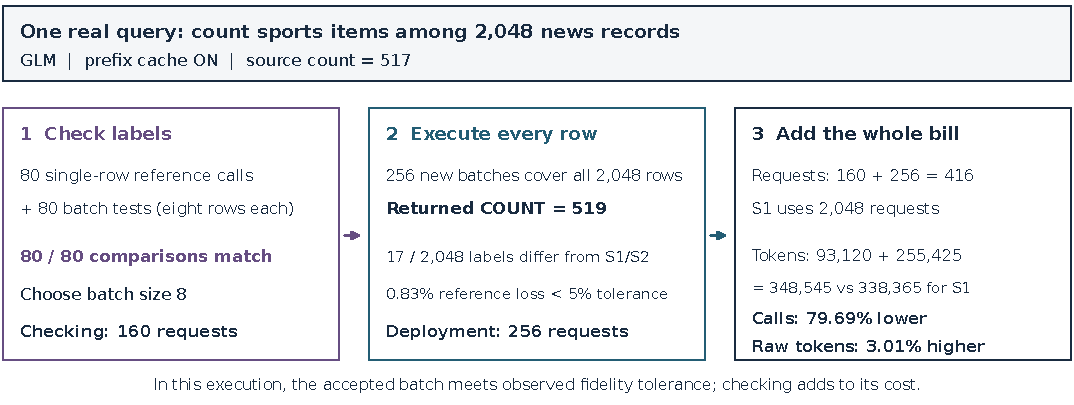
\includegraphics[width=\textwidth]{contract_execution_overview.pdf}
\caption{From a semantic COUNT query to a checked execution. The prepared review relation is the input to both checking and deployment. (a) The current-input check uses a Clopper--Pearson (CP) bound and compares one focal row per independently sampled probe batch with a singleton label. Its nominal certificate concerns agreement under that sampler. (b) Deployment labels every row once in disjoint batches, then computes COUNT outside the model. (c) We separately measure Boolean delivery and strict format, agreement with two complete singleton executions (S1/S2), COUNT error relative to the supplied-source count ($G=\sum_i g_i$), and the complete policy bill. The drawing is schematic; custom batching changes the prompt and output contract.}
\label{fig:execution}
\end{figure*}

These mechanisms have established precedents. Company studies context interference, aggregate masking of row changes and cached singleton prefixes~\cite{company}; Hassanzadeh and Subramanian measure semantic-query replay variation and cascade calibration~\cite{runvariance}. LOTUS defines optimization relative to reference algorithms~\cite{lotus}. NousDB provides the current-input fidelity check studied here and already measures calibration costs, selected sizes and efficient cached singleton execution~\cite{nousdb}. Our contribution is an empirical audit that joins the check's observations to a complete deployed result and native cost receipts in one declared engine setting. It measures how those established considerations jointly affect the plan decision.

We ask three questions:
\begin{enumerate}
\item \textbf{What is preserved?} How do delivered Booleans, strict output validity, fidelity to separate singleton executions, and COUNT accuracy against source labels differ?
\item \textbf{Does checking preserve the saving?} Do delivered batch plans stay within 5\% row disagreement with each reference while reducing complete requests and raw input-plus-output tokens? What changes with a larger checking budget?
\item \textbf{Which cost measure orders the plans?} Do raw input and native uncached-input counters favor the same plan when prefix caching is enabled?
\end{enumerate}

We execute native LOTUS filtering and deterministic COUNT with a custom multirow operator. The 36-configuration matrix spans six workloads, two domains and 512--7,600 rows using Qwen3-4B-Instruct-2507 (Qwen) and GLM-4-9B-Chat (GLM). Twelve primary configurations compare every workload at a common size/cache setting; 24 anchors vary size or cache. Sixteen follow-up policies compare 80/320-probe budgets. Complete singleton replays, deployed partitions and native receipts connect checking to results and costs.

Unchecked random and similarity batches meet the joint criterion in 1/12 and 2/12 primary configurations; the checked policy meets it in 0/12. Its sole accepted deployment preserves both observed references, but calibration consumes its raw-token saving. Larger follow-up budgets retain fallback at higher cost. Cache-enabled fixed plans favor batching on raw input and singleton execution on uncached input. Classical COUNT controls and earlier experiments place these representation-specific observations in context. The artifact preserves every configuration, negative case and resource record.\footnote{\raggedright Public materials: \url{https://github.com/yzd2002/semantic-aggregation-audit-icde2027}.}

\section{What the Query and Check Preserve}
\label{sec:objects}
\subsection{Delivered Labels and Observed References}
Let $T=(r_1,\ldots,r_N)$ be the prepared input relation. Each row occurrence has a distinct ID and its complete source-provided text field. A deployed plan labels every occurrence exactly once. A probe batch is an artificial context used for checking; probe batches can overlap and need not cover $T$ (Fig.~\ref{fig:execution}).

\emph{Native delivery} means that the engine returns a complete Boolean vector and hence a COUNT. LOTUS's native parser searches for \texttt{true} before \texttt{false} after the first \texttt{Answer:}, or in the whole response if that prefix is absent; it defaults to \texttt{True} if neither occurs. We also apply an \emph{extra strict-format check}: only a standalone Boolean, optionally prefixed by \texttt{Answer:}, is valid. Its label is $s_i\in\{0,1,\bot\}$, where $\bot$ denotes invalid format. Thus a query can deliver a native COUNT while its strict COUNT is unavailable. We report format validity, actual defaults and execution exceptions separately.

Preserved Qwen World S1 responses include \texttt{Answer: Sports} and \texttt{Answer: Sci/Tech}. Neither contains a Boolean word, so native parsing defaults to \texttt{True} while strict validity fails. The custom multirow operator instead requests a constrained JSON object mapping ordered local row IDs to \texttt{True}/\texttt{False} strings. All $k$ required labels must be valid; a missing or invalid label makes the complete vector and COUNT unavailable.

S1 and S2 are two complete native singleton executions with fresh responses, used only to evaluate completed policies. Comparing with both exposes sensitivity to the observed reference execution. The checker pays for separate calibration singleton calls; neither S1/S2 nor source labels enter selection. Held-out validation also obtains fresh singleton/batch pairs. These are observed execution references, not ground truth. For a complete policy vector $b$, its native-reference row losses are
\begin{equation}
 d_j(b)=\frac{1}{N}\sum_i\ind[b_i\ne n_i^{(j)}],\quad j=1,2,
\label{eq:fidelity}
\end{equation}
where $n_i^{(j)}$ is reference $j$'s native label. We summarize the larger loss as $d_{\max}=\max(d_1,d_2)$. Strict-vector fidelity is a separate diagnostic, available only when both full strict vectors exist; a valid subset cannot supply a full-relation COUNT.

\subsection{Source COUNT and Row Fidelity}
Supplied source labels give a separate task target. Let $g_i$ be the fixed binary source label, $G=\sum_i g_i$ the source COUNT and $C_b=\sum_i b_i$ the plan's COUNT. We report source row error and two COUNT-error units:
\begin{equation}
\begin{aligned}
 e_{\rm row}&=\frac{\sum_i\ind[b_i\ne g_i]}{N},\\
 e_N&=\frac{|C_b-G|}{N},\quad e_G=\frac{|C_b-G|}{G}\ (G>0).
\end{aligned}
\label{eq:task}
\end{equation}
$G=0$ is reported separately. The additive error $e_N$ measures error as a fraction of the input; $e_G$ measures it relative to the source-positive count. Source annotations have not been newly human-verified.

False positives (FP) raise the count and false negatives (FN) lower it. They add in row error but can cancel in COUNT error: the respective numerators are $\mathrm{FP}+\mathrm{FN}$ and $|\mathrm{FP}-\mathrm{FN}|$. Similarly, $|C_b-C_{S_j}|/N\le d_j$: a realized row-fidelity bound also bounds additive COUNT change to that same realized reference. It does not establish source accuracy or a 5\% source-relative COUNT guarantee. Our COUNT controls use the additive tolerance $.05N$.

The check targets a different object: the probability $\varphi(k)$ that a focal batch label agrees with a singleton label under a specified random row/context sampler~\cite{nousdb}. A nominal bound on this probability relies on the check's oracle and independence assumptions. It is distinct from $d_j$ for one complete deployed partition; the calibration references and later S1/S2 can also vary. We therefore report calibration, independent validation and deployment separately. Changing to similarity grouping changes the sampler again. A realized above-tolerance loss would require interpretation under these assumptions; it would not by itself establish a false certificate or a NousDB bug.

\section{Policies and the Existing Fidelity Check}
\label{sec:budget}
\subsection{Policy Key}
The fixed-plan baselines are \textbf{Random8}, a seeded random-permutation partition into batches of eight, and \textbf{Similar8}, deterministic term-frequency/inverse-document-frequency (TF--IDF) sparse-cosine greedy grouping with frozen ties. Neither performs calibration or supplies a fidelity certificate. Similar8 is a known grouping reference, rather than the full BATCHER method~\cite{batcher}; its CPU construction is charged.

The checked policies reproduce NousDB's paper-defined Algorithm~2 with a declared tested ceiling $k_{\max}=8$ supplied to the procedure~\cite{nousdb}. We evaluate this subprocedure, rather than NousDB's complete engine or histogram optimizer. Preflight retains complete fields: the longest tested eight-row prompts use 2,260 Qwen and 2,173 GLM tokens. Both plus 128 output tokens fit the 8,192-token window; a length guard also checks every submitted request. Eight is the tested ceiling, not a maximal or optimal size. Candidates are $8,4,2$ in descending order, with mismatch tolerance $\eta=.05$ and error budget $\delta=.05$. Names encode the probe budget and agreement rule:
\begin{itemize}
\item \textbf{Current80-S}, used in all 36 main configurations, permits 80 probes per candidate. Agreement requires valid strict batch and singleton labels that are equal.
\item \textbf{Current80-N} and \textbf{Current320-N}, used in the follow-up, permit 80 and 320 probes. Both require a valid batch label equal to the native singleton Boolean, including disclosed defaults. Strict reference format remains a separate diagnostic.
\end{itemize}
The S/N suffix distinguishes the strict/native agreement rule. Only the Current80-N/Current320-N contrast holds that rule fixed while changing budget. A post-hoc native-rule replay rescores only original recorded responses. It recovers selection and issued-call bills because native mismatches alone already force every observed rejection (Section~\ref{sec:budget_results}). It runs no new deployment and supplies no quality or latency measurement for an unexecuted policy.

\subsection{Check, Select and Deploy}
For a fixed input $T$ and budget $n$, the procedure is:
\begin{enumerate}
\item Draw $n$ focal row occurrences independently and uniformly from $T$, with replacement, and issue $n$ fresh singleton requests, one per probe index. Even repeated occurrences receive new calls. Reuse this indexed focal/reference sequence across this policy's candidate sizes only.
\item For each candidate $k=8,4,2$, construct each probe batch independently: sample $k-1$ other occurrences uniformly without replacement, excluding the focal occurrence, and insert it in a uniformly chosen slot. Require the entire $k$-label JSON response to be valid, then score only the focal label against its singleton reference under the chosen S/N rule.
\item Issue batch probes in chunks of 16 requests. Select the first candidate whose fixed-budget agreement bound passes, accepting only after all $n$ trials. After each whole chunk returns, score every issued trial and reject if even perfect remaining trials cannot pass; then try the next size. Every issued response is scored and billed, including the tail after a logically decisive probe.
\item Physically evaluate the frozen complete random partition at the selected size, obtaining new model responses. If no candidate passes, run fresh native singleton fallback ($k=1$). Deployment covers every occurrence once and reuses no probe responses.
\end{enumerate}
At $k=8$, the row grouping is exactly Random8's frozen grouping, evaluated through separate physical calls without reusing Random8 responses. Lower candidates use their frozen partitions. New calls preserve that layout; their statistical independence remains an assumption. Similar8's grouping is different and inherits no certificate from random probes.

Write $V_B$ for validity of the entire $k$-label batch response and $V_S$ for strict validity of its singleton reference. One trial's success indicator $Z_k$ requires $V_B$, $V_S$ and equal focal labels under S; under N it requires $V_B$ and equality to the native singleton label. Then $\varphi(k)=\Pr(Z_k=1)$ under the stated focal/context sampler and oracle assumptions. This is one focal-trial probability, not a probability that every batch label is correct.

For $X_k$ agreements out of $n$, the one-sided Clopper--Pearson (CP) lower endpoint is
\begin{equation}
\underline\varphi_k=\mathrm{Beta}^{-1}(\delta/3;X_k,n-X_k+1),
\label{eq:cp}
\end{equation}
with endpoint zero when $X_k=0$~\cite{clopper}. The threshold is $\underline\varphi_k\ge1-\eta=.95$. The $\delta/3$ allocation covers the three candidates in this one policy. Its nominal interpretation retains fixed-oracle and independent-trial assumptions; replay observations do not establish them. It supplies no joint guarantee across the matrix, probe budgets or a post-hoc selected winner.

\subsection{Why Compare Probe Budgets?}
NousDB's zero-error feasibility rule~\cite{nousdb} gives
\begin{equation}
 n_{\min}=\left\lceil\frac{\log(3/\delta)}{\log(1/(1-\eta))}\right\rceil=80.
\end{equation}
At this budget, passing requires zero disagreements; 320 probes allow seven. Under a hypothetical independent and identically distributed (IID) mismatch probability $q$, acceptance probability is $\pi_n(q)=\Pr\{\mathrm{Binomial}(n,q)\le e_{\max}(n)\}$, where $e_{\max}$ is the allowed disagreement count. At $q=.01$, it rises from .447523 to .983697. This exact binomial calculation explains the potential power gain; it is not measured model behavior. A stopped probe prefix cannot provide an unbiased estimate of $q$.

Greater power also costs more checking. Calibration uses at most $4n$ requests (singleton references and three candidate families), and deployment at most $N$, so $C_n\le4n+N$. A first-candidate $k=8$ pass uses $2n+N/8$ requests. At $N=7,600$, the 80/320 budgets therefore use 1,110/1,590 requests for that pass, or at most 7,920/8,880 with fallback. Each probe batch still reads and labels all $k$ rows. Whether more probes improve the complete bill is an empirical question.

\section{Experimental Design and Cost Accounting}
\label{sec:design}
\subsection{Queries, Inputs and Configurations}
A \emph{workload} pairs a semantic predicate with its prepared input; a \emph{configuration} fixes the workload, input size, model and cache setting. The main study has 36 configurations, each executing five methods: S1, S2, Random8, Similar8 and Current80-S. These are 36 comparison settings, not 36 model calls. The primary matrix has six workloads $\times$ two models = 12 configurations. Each extension uses three anchor workloads $\times$ two sizes $\times$ two models = 12 more. The separate budget follow-up has two workloads $\times$ two models $\times$ two budgets $\times$ two repeats = 16 complete policy executions, forming eight 80/320-budget pairs (Table~\ref{tab:matrix}).

\begin{table*}[!t]
\caption{Study design. Every listed workload/size/cache combination uses both Qwen3-4B-Instruct-2507 and GLM-4-9B-Chat. $N$ counts rows entering the semantic filter after structured filtering. The follow-up crosses two workloads, two models, two budgets and two physical repeats.}
\label{tab:matrix}
\centering\tableformat
\begin{tabular}{P{.15\textwidth}P{.38\textwidth}P{.12\textwidth}P{.10\textwidth}P{.13\textwidth}}
\toprule
\tablehead{Family} & \tablehead{Workloads} & \tablehead{Input $N$} & \tablehead{Prefix cache} & \tablehead{Count} \\
\midrule
Primary & Movie top/other critics; AG World, Sports, Business, Sci/Tech & 2,048 & ON & 12 cases \\
Scale anchors & Both Movie views; AG Sci/Tech & 512; 7,600 & ON & 12 cases \\
Cache anchors & Same three anchors & 2,048; 7,600 & OFF & 12 cases \\
\midrule
Budget follow-up & Movie other critics; AG Sci/Tech & 7,600 & ON & 16 policies \\
\bottomrule
\end{tabular}
\end{table*}

Movie has two disjoint critic views, defined by \texttt{isTopCritic=True/False}. Both ask whether the supplied \texttt{reviewText} is clearly positive. Source $g_i$ is the dataset's \texttt{scoreSentiment}: \texttt{POSITIVE} maps to one and \texttt{NEGATIVE} to zero; ``clearly positive'' is the model's question wording. The critic flag only selects the view. Neither sentiment labels nor view metadata enter inference. We use version~4 of the official SemBench generator's upstream source~\cite{sembench,movie_data}, deduplicate normalized text globally before forming the views, and fix order by a feature hash. An additional integration case runs original SemBench Movie Q3 unchanged on its official 2,000-row demonstration relation; 120 rows reach the semantic filter. The larger Movie workloads are prepared-relation COUNT variants, not scaled executions of original Q3 on the raw Reviews table.

Throughout, $N$ counts rows entering the semantic filter. The unchanged Q3 integration case is outside both the 36 main configurations and the 16 follow-up policies.

AG News uses a pinned, duplicate-free, feature-hash-ordered 7,600-row test split~\cite{agnews}. Four predicates---World, Sports, Business and Sci/Tech---share this corpus. Each frozen predicate asks for a four-topic classification and then membership in its named topic; Movie uses one clearly-positive question. We retain the complete supplied \texttt{text}/\texttt{reviewText} fields. They are not claimed to be complete original articles. Acquisition hashes and source notices are retained; AG's license remains unknown.

The frozen Sports predicate used in the running example is:
\begin{quote}\small
Classify the news item by its primary topic among World, Sports, Business, and Sci/Tech. Determine if its primary topic is Sports (sports or athletic competition). News item: \{text\}
\end{quote}
Native LOTUS also specifies: \texttt{Answer: <Your answer here. The answer should be either True or False>}. The conflicting topic-word responses are observed outcomes, not a matched causal test of this wording.

Thus six workloads span two domains and three corpus views. Shared-corpus predicates, nested sizes, cache settings and model variants are dependent observations, not independent datasets. Source membership, fields, prompts, groupings and schedules were hash-bound before their corresponding inference; no text was shortened or replaced after outcomes.

\subsection{Engine, Batching and Replays}
LOTUS v1.2.4 at a pinned commit executes live \texttt{sem\_filter} against native vLLM~\cite{vllm} through an isolated CPU process. Native execution builds one prompt per row and submits prompts concurrently. This server concurrency differs from multirow prompting. Our custom batch operator serializes each record's complete native \texttt{context\_and\_claim}, including its repeated predicate, as a JSON string with escaped newlines and quotes. It also changes system instructions and output requirements. The comparison therefore concerns these integrated physical plans; it does not isolate neighboring-text effects or test a minimum-token template that factors out the predicate.

The schematic prompt structures are: native instructions plus one complete context/claim, returning a Boolean; versus batch instructions plus $k$ serialized complete contexts/claims, including $k$ predicate copies, returning local-ID Boolean labels. These describe the representation, not new prompt variants.

Every configuration executes separate S1/S2 references, Random8, Similar8 and Current80-S. Complete plans use no training fillers and cover each input occurrence once. After a main-study non-singleton selection, 80 independently seeded validation probes receive fresh singleton and batch calls at the selected size. Validation never enters selection and is charged only to the research ledger. Random8 and Similar8 each run in all 36 main configurations, including the 12 primary ones. A separate same-size grouping comparison with Similar8 is available only for a checked $k=8$ deployment; other selections change both size and grouping. The follow-up adds no validation family.

\subsection{Follow-Up and Runtime Settings}
The follow-up fixes AG Sci/Tech and a feature-hash-selected Movie other-critics view, $N=7,600$, cache ON, two models, two budgets and two repeats: 16 complete policies. The trigger was the first Qwen AG Sci/Tech result at $N=7,600$: Current80-S fell back despite strict-valid calibration references. Sci/Tech was an existing anchor; the Movie view was chosen by the minimum seeded hash of the two existing workload IDs, yielding other critics. The fourfold budget tests whether allowing up to seven failed comparisons, instead of none, changes size selection. The follow-up was frozen before its own calls. Common feature/probe seeds pair the inputs, while all responses and deployments are physically new. Existing S1/S2 are evaluation-only. The repeats are descriptive observations on fixed inputs, not independent datasets.

Each model uses one NVIDIA GeForce RTX 5090 (32~GB; 32,607~MiB reported), PyTorch~2.8.0+cu128, vLLM~0.10.2 and Transformers~4.57.1. Qwen3-4B-Instruct-2507 and GLM-4-9B-Chat~\cite{qwen,glm} run native bfloat16 (BF16) inference with temperature zero, an 8,192-token window, eager execution, at most 32 active sequences and native/batch output caps 32/128. Effective classes, tokenizer/runtime hashes and actual cache-reset receipts are retained. The longest tested eight-row prompts use 2,260 Qwen and 2,173 GLM tokens; each plus 128 output tokens fits the window, and a guard checks every request. Raw returns are stored before parsing. There is no automatic retry, model replacement, post-label resampling or selective deletion; failures and unknown costs remain explicit.

\subsection{What Is Included in a Policy Bill?}
\label{sec:resources}
Checking is called \emph{calibration} in the execution records; the two terms denote the same phase. A request, or model call, processes one prompt. A standalone policy pays for CPU grouping, its own singleton checking references, all issued probe chunks, and complete execution at the selected size or singleton fallback. S1/S2 and independent validation score the policy for the study; they are charged to the research ledger, rather than to that standalone policy. Each policy starts with an empty prefix cache and may reuse only its own checking-to-execution prefix computation. Cache OFF is a separately executed configuration; operator and response memoization are disabled.

For requests, the accounting is simply checking plus execution: Sports uses $160+256=416$, compared with 2,048 for S1. Token accounting needs another distinction. Let $P$ be all input tokens written in requests, $O$ all generated output tokens, and $K$ the input tokens the server reports as served from its prefix cache. The totals cover the same policy phases. We retain both
\begin{equation}
\underbrace{P+O}_{\text{raw input-plus-output tokens}},\qquad
\underbrace{U=P-K}_{\text{uncached input tokens}}.
\label{eq:costs}
\end{equation}
Raw tokens count the prompt and response volume. Uncached input subtracts reused input computation and is a proxy for fresh prefill work; output generation remains separate~\cite{apc}. Neither quantity is a dollar bill or a runtime prediction. Missing cached-token counters remain unknown with bounds, rather than being replaced by zero. Sports will illustrate the complete raw-token bill; matched cache ON/OFF cases will illustrate the second cost measure.

Our primary \emph{joint benefit criterion} asks for all four conditions: (i) a complete native result; (ii) actual batching, $k>1$; (iii) at most 5\% row disagreement with each of S1/S2; and (iv) fewer requests \emph{and} fewer raw input-plus-output tokens than S1. A fallback can preserve reference labels, but it is not a successful batch deployment. Source accuracy and uncached input are reported separately. The strict-vector sensitivity evaluates the same result and bill using complete strict labels; it keeps unavailable cases in the 12-case denominator.

Elapsed time starts after a verified cache reset and includes CPU grouping, client isolation, durable tracing, transport, checking and execution. Input preparation, model loading and the reset are outside the timer. Shared-server times are descriptive; the plan comparisons below use explicit requests and token counters.

\section{Does the Checked Policy Improve the Complete Query?}
\label{sec:results}
All 36 main configurations and 16 follow-up policies completed. Figure~\ref{fig:primary} summarizes the primary matrix.\begin{figure*}[!t]
\centering
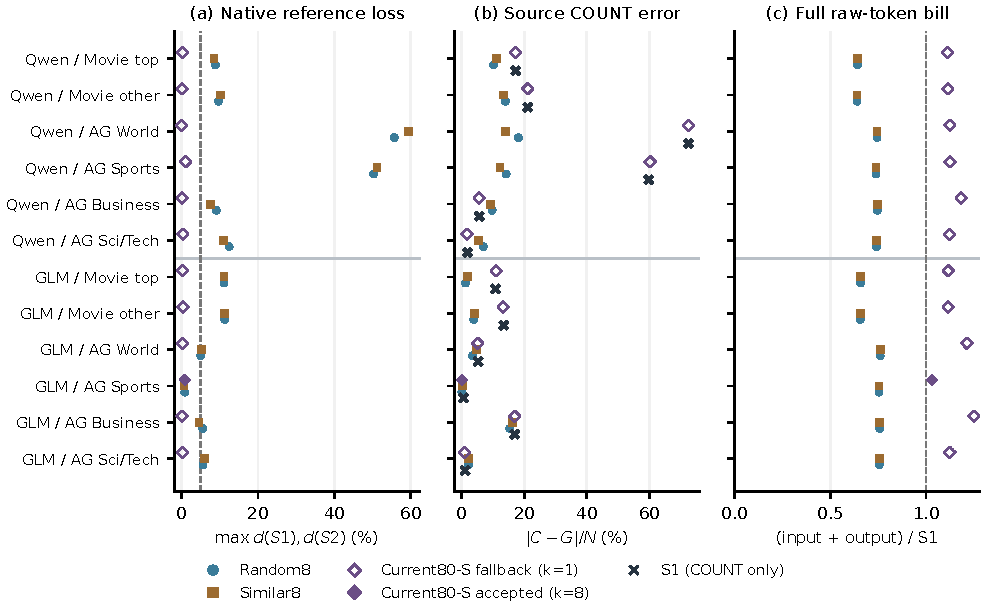
\includegraphics[width=\textwidth]{primary_execution_readouts.pdf}
\caption{All 12 primary configurations ($N=2,048$, cache ON), grouped by model. From left to right: the 0--5\% detail and full range of maximum disagreement with S1/S2; absolute source COUNT error divided by $N$; and complete input-plus-output tokens divided by S1. Smaller values are better. Dashed lines mark the 5\% reference threshold and unit cost. The two fidelity panels show the same measurements at different scales. Hollow diamonds denote fresh singleton fallback; only the filled diamond is an accepted batch. Crosses show S1's source COUNT error.}
\label{fig:primary}
\end{figure*}
 The main checker selected a batch size above one only for GLM Sports at $N=2,048$, cache ON. We follow that execution from checking to the returned count and full bill before examining the remaining outcomes.

\subsection{Walkthrough: A Passed Check and Its Full Bill}
\label{sec:sports_walkthrough}
For GLM Sports, Current80-S selected $k=8$ after all 80 calibration comparisons agreed. The separately seeded validation then found two mismatches in 80 fresh comparisons (2.5\%). Deployment labeled all 2,048 rows in 256 disjoint batches and disagreed with each complete S1/S2 reference on 17 rows (.83\%). The 80/80 checking result, the 2/80 validation result and the 17/2,048 deployment result answer separate questions. Validation is evaluation-only; it changes neither selection nor the policy bill.

The returned count was 519 against source $G=517$, giving $e_N=.10\%$ and $e_G=.39\%$, with 1.66\% source row error, as worked through in Section~\ref{sec:objects}. S1 itself had 2,025/2,048 correct source labels. This provides a usable-reference case for separating fidelity from cost. The separately executed Similar8 plan had 13/2,048 reference mismatches (.63\%); its changed grouping is an observed alternative, not an additional certificate from random probes.

Deployment alone used 256 requests and 255,425 raw input-plus-output tokens. Calibration added 160 requests and 93,120 tokens. The complete policy thus used 416 requests and 348,545 tokens, compared with S1's 2,048 requests and 338,365 tokens. Requests fell by 79.69\%, but raw tokens rose by 3.01\%. The separately executed Random8 baseline had the same observed deployment-only token bill, .754880 times S1. Charging the check consumes that saving, so the checked plan fails the joint benefit criterion despite meeting observed fidelity tolerance.

\subsection{Whole-Policy Benefit Across the Primary Matrix}
\label{sec:bill_results}
Figure~\ref{fig:primary} separates native-reference loss, source COUNT error and full raw-token cost for all 12 primary configurations. Table~\ref{tab:policy_summary} applies the fixed-denominator joint benefit criterion from Section~\ref{sec:resources}. Random8 meets both reference-loss thresholds and lowers requests and raw tokens in GLM Sports (1/12). Similar8 does so in GLM Sports and Business (2/12); Business's maximum reference loss is 4.54\%. These fixed plans have neither calibration cost nor a fidelity certificate.

\begin{table*}[!t]
\centering\tableformat
\caption{Policy comparison over the same 12 primary configurations. Benefit requires a complete result, batching, at most 5\% disagreement with both references, and fewer calls and raw tokens than S1 (Section~\ref{sec:resources}). Cost ratios use each case's S1. Strict benefit keeps all 12 cases; missing complete strict plan/reference vectors are unavailable. The fixed plans' six unavailable cases lack strict references. Source accuracy is evaluated separately.}
\label{tab:policy_summary}
\begin{tabular}{lrrrrr}
\toprule
\tablehead{Plan} & \tablehead{Max. reference loss (\%)} & \tablehead{Calls/S1} & \tablehead{Raw tokens/S1} & \tablehead{Native benefit} & \tablehead{\shortstack{Strict benefit;\\unavailable of 12}} \\
\midrule
Random8 & 0.83--55.71 & 0.125--0.125 & 0.640--0.761 & 1/12 & 1/12; 6 \\
Similar8 & 0.63--59.47 & 0.125--0.125 & 0.640--0.761 & 2/12 & 1/12; 6 \\
Current80-S & 0.00--1.12 & 0.203--1.102 & 1.030--1.251 & 0/12 & 0/12; 6 \\
\bottomrule
\end{tabular}
\end{table*}



Current80-S meets the criterion in 0/12 primary configurations, including 0/10 outside the two Qwen workloads with severe default-True parsing. The other 35 main configurations select fresh singleton fallback and pay for calibration as well as their new complete execution. No secondary size/cache configuration adds a non-singleton selection. Sports was not a preselected scale anchor, so these measurements do not identify its break-even size outside $N=2,048$.

\subsection{Reference Fidelity and Source COUNT Are Different}
\label{sec:quality_results}
The supplied labels also let us evaluate the singleton reference itself; complete per-workload baseline readouts are retained in the artifact. Qwen World and Sports triggered default-True parsing on 1,936 and 1,664 of 2,048 rows. Their native counts were 1,999 versus source $G=514$, and 1,741 versus $G=517$; source row errors were 74.37\% and 60.74\%. A post-hoc World S1 inspection found normal \texttt{stop} termination on all 2,048 calls with only 4--6 output tokens. These observations characterize the frozen two-step query wording, model and native parser together; no matched rewrite isolates the cause. Strict-format checking exposes the format issue while native COUNT remains delivered. Preserving such a reference would also preserve its task errors.

\begin{table*}[!t]
\centering\small
\caption{All 12 primary Current80-S executions ($N=2,048$, cache ON). Every case returns a native COUNT. The two count columns are integers, not a ratio. Strict-valid rows report output format; maximum reference loss compares the native result with both S1/S2. Requests and raw input-plus-output tokens include checking and full execution, divided by S1. Size one denotes fresh singleton fallback.}
\label{tab:primary_results}
\begin{tabular}{lrrrrrrr}
\toprule
Workload & $k$ & \shortstack{Strict-valid\\rows / $N$} & \shortstack{Returned\\COUNT $C_b$} & \shortstack{Source\\COUNT $G$} & \shortstack{Max. reference\\loss (\%)} & Requests/S1 & \shortstack{Raw tokens\\/ S1} \\
\midrule
\multicolumn{8}{l}{\textit{Qwen}} \\
Movie top & 1 & 2048/2,048 & 896 & 1,251 & 0.20 & 1.062 & 1.11 \\
Movie other & 1 & 2048/2,048 & 986 & 1,418 & 0.15 & 1.062 & 1.11 \\
AG World & 1 & 114/2,048 & 1,999 & 514 & 0.00 & 1.062 & 1.12 \\
AG Sports & 1 & 387/2,048 & 1,750 & 517 & 1.12 & 1.062 & 1.12 \\
AG Business & 1 & 2040/2,048 & 613 & 498 & 0.15 & 1.078 & 1.18 \\
AG Sci/Tech & 1 & 2025/2,048 & 483 & 519 & 0.34 & 1.062 & 1.12 \\
\midrule
\multicolumn{8}{l}{\textit{GLM}} \\
Movie top & 1 & 2048/2,048 & 1,025 & 1,251 & 0.24 & 1.062 & 1.12 \\
Movie other & 1 & 2048/2,048 & 1,145 & 1,418 & 0.39 & 1.062 & 1.12 \\
AG World & 1 & 2045/2,048 & 621 & 514 & 0.24 & 1.086 & 1.21 \\
AG Sports & 8 & 2048/2,048 & 519 & 517 & 0.83 & 0.203 & 1.03 \\
AG Business & 1 & 2045/2,048 & 845 & 498 & 0.10 & 1.102 & 1.25 \\
AG Sci/Tech & 1 & 2048/2,048 & 499 & 519 & 0.15 & 1.062 & 1.12 \\
\bottomrule
\end{tabular}
\end{table*}


All 12 primary Current80-S policies delivered native counts, but only six had complete strict vectors (Table~\ref{tab:primary_results}). The native joint benefit result is 0/12. The strict-vector sensitivity has zero satisfied, six evaluated-negative and six unavailable cases. Unavailable strict COUNT is distinct from native query failure.

The unchanged SemBench Q3 integration case illustrates the denominator distinction. Its 2,000-row demonstration relation sends $N=120$ rows to the semantic filter, with $G=14$. Qwen returns 7 and GLM 9 under both cache settings, without defaults and with complete strict outputs. The absolute COUNT errors are seven and five rows: $e_N=5.83\%$ and 4.17\%, but $e_G=50.00\%$ and 35.71\%. These integration measurements are separate from the larger prepared-relation variants.

\subsection{More Probes, the Same Fallback Decisions}
\label{sec:budget_results}
The follow-up holds the native-Boolean agreement rule fixed while comparing Current80-N with Current320-N. All 16 policies select singleton fallback and deliver native COUNT. Twelve have complete strict vectors; four have unavailable strict counts. Table~\ref{tab:budget_results} gives every paired comparison, and Fig.~\ref{fig:budget} separates checking from execution.

\begin{table*}[t]
\centering\small
\caption{Every paired Current80-N$\to$Current320-N follow-up ($N=7,600$, cache ON). $R$: complete requests; $d_{\max}$: maximum native row disagreement with S1/S2. Raw-token and uncached-input ratios compare complete 320-probe with 80-probe policies. Repeats are descriptive; each budget has its own nominal scope.}
\label{tab:budget_results}
\begin{tabular}{llrrrrrr}
\toprule
Model / workload & Rep. & $k$ & \shortstack{Calibration\\calls} & Full $R$ & \shortstack{Raw tokens\\$320/80$} & \shortstack{Uncached input\\$320/80$} & $d_{\max}$ (\%) \\
\midrule
Qwen / AG Sci/Tech & 1 & 1$\to$1 & 160$\to$608 & 7,760$\to$8,208 & 1.11 & 1.13 & 0.41$\to$0.36 \\
Qwen / AG Sci/Tech & 2 & 1$\to$1 & 144$\to$656 & 7,744$\to$8,256 & 1.11 & 1.12 & 0.45$\to$0.28 \\
Qwen / Movie other & 1 & 1$\to$1 & 128$\to$464 & 7,728$\to$8,064 & 1.07 & 1.09 & 0.17$\to$0.17 \\
Qwen / Movie other & 2 & 1$\to$1 & 144$\to$640 & 7,744$\to$8,240 & 1.12 & 1.17 & 0.14$\to$0.20 \\
GLM / AG Sci/Tech & 1 & 1$\to$1 & 176$\to$672 & 7,776$\to$8,272 & 1.16 & 1.21 & 0.16$\to$0.05 \\
GLM / AG Sci/Tech & 2 & 1$\to$1 & 144$\to$736 & 7,744$\to$8,336 & 1.19 & 1.25 & 0.09$\to$0.08 \\
GLM / Movie other & 1 & 1$\to$1 & 128$\to$464 & 7,728$\to$8,064 & 1.07 & 1.10 & 0.20$\to$0.20 \\
GLM / Movie other & 2 & 1$\to$1 & 176$\to$672 & 7,776$\to$8,272 & 1.15 & 1.23 & 0.20$\to$0.14 \\
\bottomrule
\end{tabular}
\end{table*}

\begin{figure*}[!t]
\centering
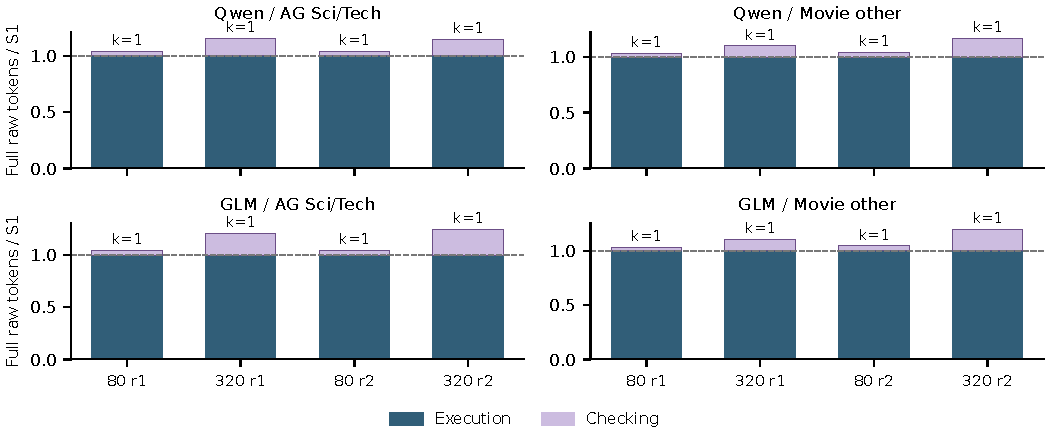
\includegraphics[width=\textwidth]{budget_full_bill.pdf}
\caption{All 16 native-rule follow-up policies ($N=7,600$, cache ON). Each pair compares 80 and 320 probes within one descriptive physical repeat. Bars include fresh calibration and complete execution, divided by the original S1 input-plus-output token bill for that input. Numbers above the bars give total cost ratios; 80 and 320 are probe budgets. Blue denotes execution and violet denotes checking. Every selected size is one. These measured costs are distinct from the hypothetical IID acceptance-power calculation.}
\label{fig:budget}
\end{figure*}

In all eight pairs, 320 probes increase full requests by 4.35--7.64\%, raw tokens by 6.82--19.20\%, and API uncached input by 8.69--25.46\%. Neither tested budget improves the deployment choice on these anchors. The hypothetical IID power calculation in Section~\ref{sec:budget} does not estimate this panel's mismatch probability. Rejecting a candidate means that the policy did not certify it, not that every possible batch is unsafe.

One recorded Qwen AG Sci/Tech pair shows where the extra requests arise ($N=7,600$, cache ON, repeat~1). At budget 80, the three candidates issue 16, 16 and 48 batch probes; the 80 singleton references are reused across them. Checking therefore costs $80+16+16+48=160$ requests. At budget 320 it costs $320+48+112+128=608$. Both policies then obtain 7,600 fresh singleton labels. Table~\ref{tab:budget_worked_pair} places this request arithmetic next to the exact token receipts. In the 80-probe first candidate, the first failure is at trial 14, but the issued 16-request chunk is fully scored and billed; detailed stopping prefixes remain in the artifact.

\begin{table}[t]
\centering\small
\caption{One measured Qwen AG Sci/Tech pair ($N=7,600$, cache ON, repeat 1). Top: requests, with probes listed at sizes 8/4/2. Each full policy adds 7,600 singleton execution calls to checking. Bottom: complete token receipts; $P$ is raw input, $O$ output, $K$ cached input and $U=P-K$.}
\label{tab:budget_worked_pair}
\begin{tabular}{rrrrr}
\toprule
Budget & \shortstack{Singleton\\references} & \shortstack{Batch probes\\8 / 4 / 2} & \shortstack{Checking\\calls} & \shortstack{Full\\calls} \\
\midrule
80 & 80 & 16 / 16 / 48 & 160 & 7,760 \\
320 & 320 & 48 / 112 / 128 & 608 & 8,208 \\
\bottomrule
\end{tabular}
\par\smallskip
\begin{tabular}{rrrrr}
\toprule
Budget & $P$ & $O$ & $K$ & $U$ \\
\midrule
80 & 1,336,641 & 32,108 & 498,816 & 837,825 \\
320 & 1,483,830 & 36,842 & 533,440 & 950,390 \\
\bottomrule
\end{tabular}
\end{table}


The retained stopping-audit CSV records every observed candidate prefix. The main study observes 106 candidate prefixes (105 rejections, one pass); the follow-up observes 48 rejections. At every rejected candidate prefix, accumulated native-Boolean mismatches alone make passing impossible. Qwen also has 31 probe-level strict-only format flags, classified after excluding batch failures and native mismatches. These flags do not mean that format alone caused a candidate stop. No issued probe has a batch-contract failure. The two lower candidates after the Sports pass remain unobserved. Stopped prefixes estimate neither population mismatch probability nor a false-rejection rate.


\subsection{Cache Counters Reverse the Input-Cost Ranking}
\label{sec:cache_results}
All 48 cache-ON fixed-plan executions (24 configurations, two plans) use less raw input but more API uncached input than their own S1. Qwen's ratios are .626--.739 for raw input versus 1.083--1.157 for uncached input; GLM's are .649--.758 versus 1.142--1.285. All 24 cache-OFF fixed-plan executions favor batching on both counters. Table~\ref{tab:cache_costs} keeps raw input, output and uncached input separate, while Fig.~\ref{fig:cache} shows matched examples.

\begin{figure*}[!t]
\centering
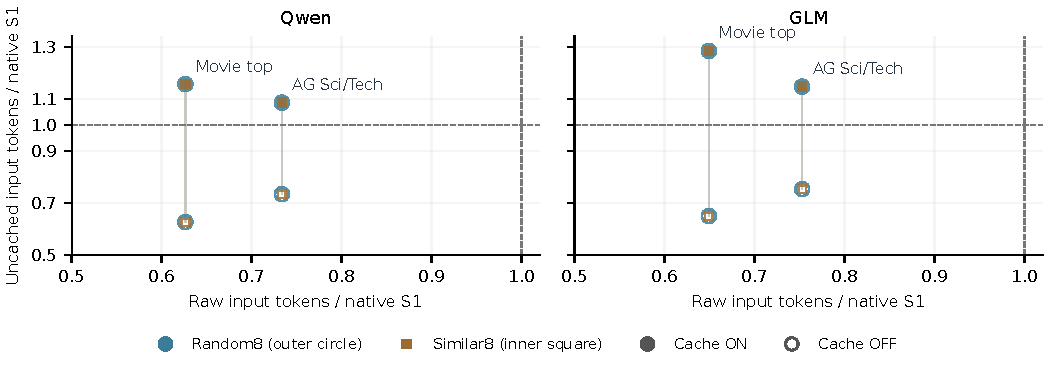
\includegraphics[width=\textwidth]{cache_input_cost_objects.pdf}
\caption{Raw versus API uncached input for Movie top and AG Sci/Tech at $N=7,600$. Lines connect matched cache-OFF/ON executions under each model. Ratios use the corresponding singleton S1 counter; one marks equal cost. Blue Random8 circles and orange Similar8 squares show coincident counters without jitter. Filled markers denote cache ON; hollow markers denote cache OFF. The upper shaded region has fewer raw input tokens but more uncached input than S1. Complete-matrix ranges are in Table~\ref{tab:cache_costs}. Uncached input is a prefill-work proxy.}
\label{fig:cache}
\end{figure*}
\begin{table*}[!t]
\centering\tableformat
\caption{Fixed-plan cost ratios to the corresponding separately executed S1. Cells give complete-matrix ranges; ON has 12 and OFF six configurations per model/plan. The last column counts raw-input ratio $P/P_{S1}<1$ but uncached-input ratio $U/U_{S1}>1$. Input, output and uncached input are distinct; uncached input is a prefill-work proxy.}
\label{tab:cache_costs}
\begin{tabular}{llrrrrr}
\toprule
\tablehead{Model/cache} & \tablehead{Plan} & \tablehead{Cases} & \multicolumn{3}{c}{\tablehead{Cost ratio to singleton S1}} & \tablehead{Reversals} \\
\cmidrule(lr){4-6}
 & & & \tablehead{Raw input} & \tablehead{Output} & \tablehead{Uncached input} & \shortstack{$P/P_{S1}<1$,\\$U/U_{S1}>1$} \\
\midrule
Qwen/ON & Random8 & 12 & 0.63--0.74 & 0.98--1.11 & 1.08--1.16 & 12/12 \\
Qwen/ON & Similar8 & 12 & 0.63--0.74 & 0.97--1.09 & 1.08--1.16 & 12/12 \\
Qwen/OFF & Random8 & 6 & 0.63--0.73 & 1.06--1.08 & 0.63--0.73 & 0/6 \\
Qwen/OFF & Similar8 & 6 & 0.63--0.73 & 1.06--1.08 & 0.63--0.73 & 0/6 \\
\midrule
GLM/ON & Random8 & 12 & 0.65--0.76 & 0.85--0.85 & 1.14--1.28 & 12/12 \\
GLM/ON & Similar8 & 12 & 0.65--0.76 & 0.85--0.85 & 1.14--1.28 & 12/12 \\
GLM/OFF & Random8 & 6 & 0.65--0.75 & 0.85--0.85 & 0.65--0.75 & 0/6 \\
GLM/OFF & Similar8 & 6 & 0.65--0.75 & 0.85--0.85 & 0.65--0.75 & 0/6 \\
\bottomrule
\end{tabular}
\end{table*}


All 24 matched anchor/size/model/fixed-plan comparisons have identical raw input counts with cache ON and OFF. In the running cache-ON Sports case, S1 writes 328,125 input tokens and reuses 131,008, leaving $U=197,117$. Random8 writes fewer inputs (246,721) but reuses only 20,400, leaving $U=226,321$. Its smaller prompt total therefore requires more uncached input. This comparison concerns input processing; the complete raw-token bill also includes output tokens. Output ratios remain separate: .974--1.106 for Qwen and approximately .850 for GLM with cache ON. These are counter rankings for the declared representation, not universal time or monetary advantages.


\clearpage
\section{Classical Controls for a COUNT-Only Goal}
\label{sec:finite}
A COUNT-only application can tolerate row errors that cancel, or estimate the count without first labeling every row. We include established finite-population controls with three reported outputs: accept/reject the unchanged COUNT; accept/reject row accuracy; or estimate COUNT directly with an interval and midpoint. These offline controls use supplied source labels, or a recorded singleton vector where available, as a fixed target $y$. Label lookups count as oracle queries; we do not price them as online model or human judgments.

The main source-label analysis requires a complete \emph{plan strict vector}: all 72 fixed-plan vectors and 26 Current80-S vectors qualify, yielding 98 pairs over the 36 configurations. Source labels are already complete; this eligibility does not require a strict singleton reference. Strict-reference fidelity in Section~\ref{sec:objects}, by contrast, requires both strict plan and reference vectors. A post-hoc source-label sensitivity uses all 108 native plan vectors with the same sample order and fixed look. These eligibility counts do not change the 36-configuration study denominator. Dependence during generation does not invalidate design-based sampling of the fixed vector pair~\cite{worcs}; the guarantee concerns that pair, not another replay or correctness beyond supplied annotations.


\subsection{Auditing a Complete Plan}
For a complete realized binary plan vector $b$, take one simple random sample without replacement of $m=\min(1,024,N)$ target labels. All procedures use this one fixed look, with tolerance $\epsilon=.05$ and error budget $\alpha=.05$. For context, the standard difference estimator $C_b-N\overline{(b-y)}_{\rm sample}$ adjusts COUNT using sampled errors, following SampleClean/control-variate approximate query processing (AQP)~\cite{sampleclean,blazeit}. It is background lineage, not a corrected-count result in our tables. Our \emph{raw-COUNT gate} asks whether uncorrected $C_b$ is already within $\epsilon N$ of the target.

To construct that gate, divide the plan into predicted-positive and predicted-negative strata. First take the overall random sample, then condition on its observed stratum sample sizes. In stratum $h$, $N_h$ is population size, $F_h$ total errors, $m_h$ sampled rows and $X_h$ sampled errors. The hypergeometric (HG) law is $X_h\sim\mathrm{HG}(N_h,F_h,m_h)$. Errors are false positives in the positive stratum and false negatives in the negative stratum. Inversion gives population \emph{error-count} intervals $[L_+,U_+]$ and $[L_-,U_-]$, in rows. Allocate $\alpha/H$ to each of $H$ nonempty strata, split across two tails. Empty strata contribute zero; an unsampled nonempty stratum retains $[0,N_h]$. A sole nonempty stratum uses full $\alpha$.

On the same joint event, intervals for signed COUNT error and total row error are
\begin{equation}
 I_\Delta=[L_+-U_-,U_+-L_-],\quad
 I_{\rm row}=[L_++L_-,U_++U_-].
\end{equation}
The raw-COUNT gate passes if $I_\Delta\subseteq[-\epsilon N,\epsilon N]$; the \emph{joint-strata row gate} passes if $\sup I_{\rm row}\le\epsilon N$. A separate direct row baseline inverts an unstratified two-sided HG interval for sample mismatches; neither row method is claimed uniformly tighter.


\subsection{Estimating COUNT Directly}
Direct AQP samples the target labels without requiring a complete batch vector. It independently inverts the sample's target-positive count to obtain a two-sided HG interval, reports the midpoint, and checks interval width $\le2\epsilon N$. It costs $m$ oracle queries and no full batch inference, so remains defined even if a batch plan cannot return a complete vector.

Each method/vector pair has a separate nominal 95\% scope. The single look is not repeatedly inspected until passing~\cite{bargain,worcs}, and selecting a favorable method or plan afterward does not preserve joint 95\% coverage. An S1-based decision evaluated against S2 is a replay sensitivity, not a coverage failure against S1. Both COUNT-error normalizations are reported, while the gates use additive $.05N$ throughout.

\section{Reproducibility and Research Accounting}
\label{sec:repro}
The public artifact contains acquisition records, frozen prompts and partitions, raw responses, request/cache receipts, native/strict vectors, exact CSVs, plotting code and source-build instructions. CPU reconstruction verifies the execution chains and complete bills without new judgments. Rescoring the main study's recorded responses under the native agreement rule recovers the same selections and issued-call costs in all 36 cases; it adds no unexecuted deployment outcome.

The successful-run research ledger records 557,996 calls: 429,584 main-study, 127,712 follow-up, 160 independent-validation, 480 original-Q3 and 60 format-control calls. Their totals are 98,862,260 input and 3,576,771 output tokens. The earlier supporting studies are separate. The policy tables exclude evaluation-only S1/S2 and validation from the policy bill. Three retained failed starts returned zero, zero and ten requests, with initialization work unmetered. The ten returns add 814 input and 62 output tokens, making 558,006 returned requests across successful and failed attempts. Full reconciliation and integrity checks are retained with the records.

Materials and run instructions are available in the \href{https://github.com/yzd2002/semantic-aggregation-audit-icde2027}{public repository}.

\section{Related Work}
BATCHER explores grouping and demonstrations for entity resolution~\cite{batcher}; BatchPrompt studies ordering, ensembles and early stopping~\cite{batchprompt}; multi-instance processing separates instance count from context length~\cite{mip}. Company distinguishes neighboring-text and prior-verdict channels, shows aggregate masking of row changes and discusses cached singleton prefixes~\cite{company}. Hassanzadeh and Subramanian measure row/COUNT changes, repetition and cascade calibration in semantic queries~\cite{runvariance}. These precedents motivate the present controls; our live plan comparison additionally changes serialization and output contracts.

Guarantees also differ in their preservation targets. LOTUS optimizes relative to reference algorithms~\cite{lotus}; SUPG targets precision/recall using proxies and oracle samples~\cite{supg}. BARGAIN develops guaranteed LLM cascades, including adaptive sampling without replacement and valid sample reuse~\cite{bargain}. NousDB supplies the independent-probe current-input CP procedure reproduced here~\cite{nousdb}. Its Table~3 already reports Certified/Batched token/runtime costs, Fig.~11 reports calibration and small selected sizes, and \S5.2 discusses continuous batching and prefix caching for efficient per-row execution. Our contribution is the joined execution audit of that paper-defined subprocedure under the declared maximum size, agreement rule and deployment representation.

The COUNT controls follow established AQP. SampleClean's NormalizedSC corrects a full dirty-data result using a cleaned sample and also supports direct clean-sample estimation~\cite{sampleclean}. BlazeIt uses aggregation control variates~\cite{blazeit}; ABAE uses proxy strata and sample allocation for expensive predicates~\cite{abae}. ThalamusDB combines model predicates, partial evaluation and query rewrites for deterministic approximate-query bounds~\cite{thalamus}, with a different complete-model target and bound construction. Finite-population inference and confidence sequences address fixed populations sampled without replacement~\cite{worcs}; the present controls use one fixed look.

SemBench measures real engines' source-defined COUNT quality, cost, latency and scale~\cite{sembench}. We retain original Q3 as an integration case and identify the larger inputs as source-derived variants. The empirical focus is how fidelity checking, a complete deployed plan and its complete bill interact when cache state and probe budget are measured explicitly.

The artifact also retains earlier context-replacement and development-transfer replications on DBLP--ACM, BoolQ and SNLI with Qwen, SmolLM2 and GLM~\cite{leipzig2010,deepmatcher,boolq,snli,smol}. Their results remain separate from the 36 live configurations and the budget follow-up.

\section{Implications and Scope}
The execution record supports two optimizer decisions: name the preservation target, then compare the complete bill under the actual cache state. Native-reference fidelity, reusable row labels and source COUNT call for different checks. COUNT-only applications can compare aggregate controls and direct AQP under their oracle requirements. A cost catalog should retain requests, input, output, cache receipts and all checking phases: calibration changes the Sports raw-token decision, while cache state changes the fixed plans' input-cost ordering.

The measured scope is two local models, six fixed predicates, two domains and three prepared views. Shared AG records, nested sizes and descriptive budget repeats retain their dependencies. The Qwen panels characterize the frozen wording/model/parser combination jointly. Batching repeats each complete context/claim and predicate while changing JSON serialization, system instructions and output requirements. Its cache ordering is therefore specific to this representation; factored templates and isolated context-interference effects require separate comparisons. The accepted deployment meets observed tolerance, leaving certificate transport failure unobserved.

Fixed-vector intervals refer to supplied annotations and their named immutable vectors. Each nominal 95\% procedure has its stated per-pair scope, separate from winner selection or future replays. Uncached input measures a prefill-work proxy; shared-server timing includes tracing and isolated clients. These resource objects support the reported plan comparisons, with monetary cost, general latency and a full NousDB optimizer comparison outside the measured scope.

\section{Conclusion}
The study connects fidelity checking to complete query results and resource bills. Fixed plans meet the joint reference-and-cost criterion in a few primary configurations; the checked policy meets it in none, including its fidelity-preserving Sports deployment. Larger probe budgets retain fallback and raise costs on the follow-up. Native cache counters reverse raw-input ordering for the declared cache-enabled fixed plans. The execution record enables reproducible comparisons of preservation targets and complete policy costs.

\label{body:end}
\clearpage
\IEEEtriggeratref{15}
\begin{thebibliography}{99}
\bibitem{batcher} M. Fan, X. Han, J. Fan, C. Chai, N. Tang, G. Li, and X. Du, ``Cost-effective in-context learning for entity resolution: A design space exploration,'' in \emph{Proc. ICDE}, 2024, pp.3696--3709, doi:10.1109/ICDE60146.2024.00284.
\bibitem{batchprompt} J. Lin, M. Diesendruck, L. Du, and R. Abraham, ``BatchPrompt: Accomplish more with less,'' in \emph{Proc. ICLR}, 2024. [Online]. Available: \url{https://proceedings.iclr.cc/paper_files/paper/2024/hash/5d8c01de2dc698c54201c1c7d0b86974-Abstract-Conference.html}
\bibitem{mip} J. Chen, M. T. Pilehvar, and J. Camacho-Collados, ``Understanding LLM performance degradation in multi-instance processing: The roles of instance count and context length,'' in \emph{Proc. ACL}, 2026, pp.31851--31884, doi:10.18653/v1/2026.acl-long.1470.
\bibitem{company} P. Xie and A. Alanwar, ``Judged in company: In-context batching makes LLM verdicts depend on other items,'' arXiv:2610.40241v1, 2026. [Online]. Available: \url{https://arxiv.org/html/2610.40241v1}
\bibitem{lotus} L. Patel, S. Jha, M. Pan, H. Gupta, P. Asawa, C. Guestrin, and M. Zaharia, ``Semantic operators and their optimization: Enabling LLM-based data processing with accuracy guarantees in LOTUS,'' \emph{Proc. VLDB Endow.}, vol.18, no.11, pp.4171--4184, 2025, doi:10.14778/3749646.3749685.
\bibitem{nousdb} C. Tsapelas, G. Koutrika, and Y. Ioannidis, ``NousDB: A fast query engine for semantic analytics,'' arXiv:2610.28551v2, 2026. [Online]. Available: \url{https://arxiv.org/html/2610.28551v2}
\bibitem{sembench} J. Lao \emph{et al.}, ``SemBench: A benchmark for semantic query processing engines,'' \emph{Proc. VLDB Endow.}, vol.19, no.8, pp.1754--1767, 2026, doi:10.14778/3811243.3811249.
\bibitem{runvariance} O. Hassanzadeh and D. Subramanian, ``Same query, different answer: Run-to-run variance in semantic query processing,'' arXiv:2610.13823, 2026.
\bibitem{qwen} Qwen, ``Qwen3-4B-Instruct-2507,'' model card, 2025. [Online]. Available: \url{https://huggingface.co/Qwen/Qwen3-4B-Instruct-2507}
\bibitem{smol} Hugging Face, ``SmolLM2-1.7B-Instruct,'' model card, 2024. [Online]. Available: \url{https://huggingface.co/HuggingFaceTB/SmolLM2-1.7B-Instruct}
\bibitem{glm} Z.ai / THUDM, ``GLM-4-9B-Chat,'' model card, 2024. [Online]. Available: \url{https://huggingface.co/zai-org/glm-4-9b-chat}
\bibitem{leipzig2010} H. K\"opcke, A. Thor, and E. Rahm, ``Evaluation of entity resolution approaches on real-world match problems,'' \emph{Proc. VLDB Endow.}, vol.3, no.1, pp.484--493, 2010, doi:10.14778/1920841.1920904.
\bibitem{deepmatcher} DeepMatcher project, ``DeepMatcher: Datasets,'' captured DBLP--ACM release. [Online]. Available: \url{https://github.com/anhaidgroup/deepmatcher/blob/master/Datasets.md}
\bibitem{boolq} C. Clark, K. Lee, M.-W. Chang, T. Kwiatkowski, M. Collins, and K. Toutanova, ``BoolQ: Exploring the surprising difficulty of natural yes/no questions,'' in \emph{Proc. NAACL-HLT}, 2019, pp.2924--2936, doi:10.18653/v1/N19-1300.
\bibitem{snli} S. R. Bowman, G. Angeli, C. Potts, and C. D. Manning, ``A large annotated corpus for learning natural language inference,'' in \emph{Proc. EMNLP}, 2015, pp.632--642, doi:10.18653/v1/D15-1075.
\bibitem{vllm} W. Kwon \emph{et al.}, ``Efficient memory management for large language model serving with PagedAttention,'' in \emph{Proc. SOSP}, 2023, pp.611--626, doi:10.1145/3600006.3613165.
\bibitem{sampleclean} J. Wang, S. Krishnan, M. J. Franklin, K. Goldberg, T. Milo, and T. Kraska, ``A sample-and-clean framework for fast and accurate query processing on dirty data,'' in \emph{Proc. SIGMOD}, 2014, pp.469--480, doi:10.1145/2588555.2610505.
\bibitem{supg} D. Kang, E. Gan, P. Bailis, T. Hashimoto, and M. Zaharia, ``Approximate selection with guarantees using proxies,'' \emph{Proc. VLDB Endow.}, vol.13, no.11, pp.1990--2003, 2020, doi:10.14778/3407790.3407804.
\bibitem{blazeit} D. Kang, P. Bailis, and M. Zaharia, ``BlazeIt: Optimizing declarative aggregation and limit queries for neural network-based video analytics,'' \emph{Proc. VLDB Endow.}, vol.13, no.4, pp.533--546, 2019, doi:10.14778/3372716.3372725.
\bibitem{abae} D. Kang, J. Guibas, P. Bailis, T. Hashimoto, Y. Sun, and M. Zaharia, ``Accelerating approximate aggregation queries with expensive predicates,'' \emph{Proc. VLDB Endow.}, vol.14, no.11, pp.2341--2354, 2021, doi:10.14778/3476249.3476285.
\bibitem{thalamus} S. Jo and I. Trummer, ``ThalamusDB: Approximate query processing on multi-modal data,'' \emph{Proc. ACM Manag. Data}, vol.2, no.3, Art.186, 2024, doi:10.1145/3654989.
\bibitem{bargain} S. Zeighami, S. Shankar, and A. Parameswaran, ``Cut costs, not accuracy: LLM-powered data processing with guarantees,'' arXiv:2509.02896v1, 2025. [Online]. Available: \url{https://arxiv.org/html/2509.02896v1}
\bibitem{worcs} I. Waudby-Smith and A. Ramdas, ``Confidence sequences for sampling without replacement,'' in \emph{Advances in Neural Information Processing Systems}, vol.33, 2020. [Online]. Available: \url{https://arxiv.org/abs/2006.04347}
\bibitem{clopper} C. J. Clopper and E. S. Pearson, ``The use of confidence or fiducial limits illustrated in the case of the binomial,'' \emph{Biometrika}, vol.26, no.4, pp.404--413, 1934, doi:10.1093/biomet/26.4.404.
\bibitem{agnews} X. Zhang, J. Zhao, and Y. LeCun, ``Character-level convolutional networks for text classification,'' in \emph{Advances in Neural Information Processing Systems}, 2015. Dataset snapshot: \url{https://huggingface.co/datasets/fancyzhx/ag_news}, revision \texttt{eb185aa}.
\bibitem{movie_data} andrezaza, ``Massive Rotten Tomatoes Movies \& Reviews,'' Kaggle dataset, version 4, CC0. [Online]. Available: \url{https://www.kaggle.com/datasets/andrezaza/clapper-massive-rotten-tomatoes-movies-and-reviews}
\bibitem{apc} vLLM project, ``Automatic prefix caching,'' v0.10.2 documentation. [Online]. Available: \url{https://docs.vllm.ai/en/v0.10.2/features/automatic_prefix_caching.html}
\end{thebibliography}

\clearpage
\section*{Acknowledgments}
\textbf{AI-generated content disclosure.} The authors retain intellectual and editorial responsibility for the research conception, overall design, and main manuscript. OpenAI Codex substantially assisted study planning, literature checks, experimental code, figure design and rendering, data analysis, and drafting and revision across all sections. Inference models and their experimental roles are documented in Section~\ref{sec:design} and the artifact. The authors take full responsibility for the content of the manuscript, including any text generated or polished by the LLM, and for ensuring originality, proper attribution, ethical compliance, and the absence of plagiarism or scientific misconduct.

\end{document}
